% --- Program Section ---

\newprogram{Program 5}{Implement fractional-knapsack(weights: List[int], values: List[int], capacity: int)
-> float and job-scheduling(jobs: List[Job]) -> List[int] functions returning maximum
attainable profit and optimal job sequence.}

\subsection*{Code}
\begin{lstlisting}[language=Python]
from typing import List
from dataclasses import dataclass

@dataclass
class Job:
    id: int
    deadline: int
    profit: int

def fractional_knapsack(weights: List[int], values: List[int], capacity: int) -> float:
    # Calculate value/weight ratio
    items = [(values[i] / weights[i], weights[i], values[i])
             for i in range(len(weights))]

    # Sort by highest value/weight ratio
    items.sort(reverse=True)

    total_profit = 0.0

    for ratio, weight, value in items:
        if capacity == 0:
            break

        if weight <= capacity:
            total_profit += value
            capacity -= weight
        else:
            # Take only the fraction that fits
            total_profit += ratio * capacity
            capacity = 0

    return total_profit

def job_scheduling(jobs: List[Job]) -> List[int]:
    # Sort jobs by decreasing profit
    jobs.sort(key=lambda job: job.profit, reverse=True)

    max_deadline = max(job.deadline for job in jobs)

    # Time slots
    slots = [None] * (max_deadline + 1)

    # Schedule jobs
    for job in jobs:
        for slot in range(job.deadline, 0, -1):
            if slots[slot] is None:
                slots[slot] = job.id
                break

    # Return scheduled job IDs
    return [job_id for job_id in slots[1:] if job_id is not None]


# -----------------------------
# Fractional Knapsack Example
# -----------------------------

weights = [10, 20, 30]
values = [60, 100, 120]
capacity = 50

print("Maximum profit:",
      fractional_knapsack(weights, values, capacity))

# -----------------------------
# Job Scheduling Example
# -----------------------------

jobs = [
    Job(1, 2, 100),
    Job(2, 1, 19),
    Job(3, 2, 27),
    Job(4, 1, 25),
    Job(5, 3, 15)
]

print("Optimal job sequence:",
      job_scheduling(jobs))
\end{lstlisting}

\subsection*{Output}
\begin{center}
    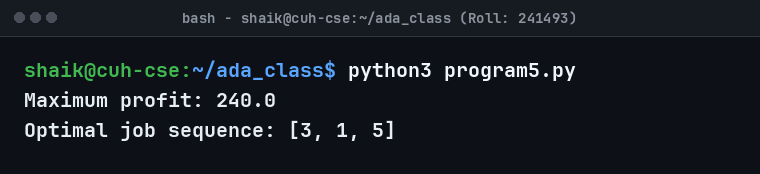
\includegraphics[width=0.88\textwidth]{Images/output_screenshot5.png}
\end{center}

\subsection*{GitHub Scan Code}
\begin{center}
    \begin{minipage}{0.3\textwidth}
        \centering
        % Generates a 2.5cm high QR code directly linking to the code file
        \qrcode[height=3.5cm]{https://github.com/gytdrop/ada_class/blob/main/program5.py} \\[0.2cm]
        \scriptsize\ttfamily Scan to view source code 
    \end{minipage}
\end{center}


% Add a horizontal line that indicates the END of the program.
\vspace{1cm}
\begin{center}
    \rule{1\textwidth}{1pt} % Clean, centered 1pt thick horizontal line
\end{center}